%% LyX 2.3.6.1 created this file.  For more info, see http://www.lyx.org/.
%% Do not edit unless you really know what you are doing.
\documentclass[english]{article}
\usepackage[T1]{fontenc}
\usepackage[latin9]{inputenc}
\usepackage{float}
\usepackage{amstext}
\usepackage{graphicx}

\makeatletter

%%%%%%%%%%%%%%%%%%%%%%%%%%%%%% LyX specific LaTeX commands.
%% Because html converters don't know tabularnewline
\providecommand{\tabularnewline}{\\}
\floatstyle{ruled}
\newfloat{algorithm}{tbp}{loa}
\providecommand{\algorithmname}{Algorithm}
\floatname{algorithm}{\protect\algorithmname}

\makeatother

\usepackage{babel}
\begin{document}
\title{Use RBF as a sampling method in Multistart global optimization method}
\author{Ioannis G. Tsoulos$^{(1)}$\thanks{Corresponding author. Email: itsoulos@uoi.gr},
Alexandros Tzallas$^{(1)}$, Dimitrios Tsalikakis$^{(2)}$}
\date{$^{(1)}$Department of Informatics and Telecommunications, University
of Ioannina, 47100 Arta, Greece \\
$^{(2)}$University of Western Macedonia, Department of Engineering
Informatics and Telecommunications, Greece}
\maketitle
\begin{abstract}
In this paper, a new sampling technique is proposed that can be used
in the Multistart global optimization technique as well as techniques
based on it. The new method takes a limited number of samples from
the objective function and then uses them to train an RBF neural network.
Subsequently, several samples were taken from the artificial neural
network this time, and those with the smallest network value in them
are used in the global optimization method. The proposed technique
was applied to a wide range of objective functions from the relevant
literature and the results were extremely promising.
\end{abstract}
\textbf{Keywords}: Global optimization, stochastic methods, termination
rules.

\section{Introduction }

A novel method to draw samples for global optimization methods is
presented here. The process of locating the global minimum of a continuous
and differentiable function $f:S\rightarrow R,S\subset R^{n}$ is
described as, determine 
\begin{equation}
x^{*}=\mbox{arg}\min_{x\in S}f(x)\label{eq:eq1}
\end{equation}
with $S$: 
\[
S=\left[a_{1},b_{1}\right]\otimes\left[a_{2},b_{2}\right]\otimes\ldots\left[a_{n},b_{n}\right]
\]
The above problem is commonly used to describe problems in economics
\cite{global_econ1,global_econ2,global_econ3}, physics \cite{global_physics1,global_physics2,global_physics3},
chemistry \cite{global_chemistry1,global_chemistry2,global_chemistry3},
medicine \cite{global_med1,global_med2} etc. The global optimization
methods have two major categories: deterministic and stochastic methods.
 The most common methods of the first category are the so-called Interval
methods \cite{interval1,interval2,interval3}, where the set $S$
is divided iteratively in subregions and some subregions that do not
contain the global solution are discarded using some pre-defined criteria.
The majority of the methods belong to the second category where the
reader can find Controlled Random Search methods \cite{crs1,crs2,crs3},
Simulated Annealing methods \cite{simann_major,simann1}, Differential
Evolution methods \cite{de1,de2}, Genetic algorithms \cite{ga1,ga2,ga3},
Particle Swarm optimization methods \cite{pso1,pso2}, Ant Colony
methods \cite{aco1,aco2} etc. Also, many hybrid stochastic methods
have appeared recently in the relevant literature. such as methods
that combine Particle Swarm Optimization and Simulated Annealing \cite{pso_sa_hybrid1,pso_sa_hybrid2},
methods that combine Genetic Algorithms and Differential Evolution
\cite{ga_de_hybrid1,ga_de_hybrid2}, combinations of Genetic Algorithms
and Particle Swarm Optimization \cite{ga_pso_hybrid1} etc. Also,
due to the wide spread of parallel architectures in recent years as
well as the widespread use of GPUs, many methods have emerged that
exploit such architectures \cite{gpu1,gpu2,gpu3}. 

This paper proposes an innovative sampling technique for the Multistart
stochastic global sampling method. The Multistart technique is one
of the simplest stochastic global optimization techniques and is the
basis for many modern global optimization methods. In the Multistart
method, a series of random samples are taken from the objective function
and then a local optimization method is started from each sample.
Regarding its simplicity, the method has been used with success in
a wide area of practical applications, such as the TSP problem\textbf{
}\cite{multistart-tsp}, the vehicle routing problem \cite{multistart-vehicle},
the facility location problem \cite{multistart_fac}, the maximum
clique problem \cite{multistart_clique}, the maximum fire risk insured
capital problem \cite{multistart_fire}, aerodynamic shape problems
\cite{multistart-aero} etc. In addition, the Multistart method has
been thoroughly studied by many researchers in recent years, and many
works have been proposed on this method, such as methods for finding
all local minima of a function \cite{tmlsl,Salhi,minfinder}, hybrid
techniques \cite{mshybrid1,mshybrid2}, GRASP methods\cite{grasp},
new termination rules \cite{msstop1,msstop2,msstop3}, parallel techniques\cite{parallel-multistart,parallel-multistart2}.
Usually, in the Multistart method, samples are used from the objective
function using some distribution such as the uniform distribution.
In the present work, it is proposed that these samples are obtained
from a radial basis network \cite{rbf1} (RBF), which has already
been trained on a limited number of real samples from the objective
function. RBF networks have been widely used in many real world problems,
such as face recognition \cite{rbf_face}, function approximation
\cite{rbf_function}, image classification \cite{rbf_image}, water
quality prediction \cite{rbf_water} etc.

The rest of this article is organized as follows: in section \ref{sec:Method-description}
the proposed sampling technique is outlined in detail, in section
\ref{sec:Experiments} the test functions used as well the experimental
results are listed and finally in section \ref{sec:Conclusions} some
conclusions are presented.

\section{Method description \label{sec:Method-description}}

\subsection{The Multistart method}

A commonly used representation of the Multistart method is shown in
Algorithm \ref{alg:multistart_typical}. In practice, the method takes
N samples at each iteration and starts a local minimization method
for each sample, without doing any other checking. However, despite
its simplicity, it has two key components which, with proper adaptation,
can make the method extremely efficient. The first component is the
termination method used and the second is the sampling method within
the central iteration. The local search procedure used here is an
adaptation of the BFGS method \cite{powell}. The used termination
rule was also used in a variety of global optimization methods \cite{ga_tsoulos,pso_tsoulos}.
This termination method is outlined in subsection \ref{subsec:The-used-termination}
The second point, which this paper focuses on, is the sampling method.
Usually, sampling is done with random samples from some distribution
such as the uniform one. In this paper, samples will be taken from
an approximation of the objective function $f(x)$ constructed using
an RBF neural network. This approach is discussed in subsection \ref{subsec:Rbf-networks}.

\begin{algorithm}
\caption{Representation of the Multistart algorithm.\label{alg:multistart_typical}}

\begin{enumerate}
\item \textbf{Initialization} step.
\begin{enumerate}
\item \textbf{Set} $N$ the number of samples, that will taken in every
iteration.
\item \textbf{Set} $\mbox{ITER}_{\mbox{MAX}}$, the maximum number of allowed
iterations.
\item \textbf{Set} Iter=0, the iteration number.
\item \textbf{Set} $\left(x^{*},y^{*}\right)$ as the global minimum. Initialy
$y^{*}=\infty$
\end{enumerate}
\item \textbf{Evaluation} step.
\begin{enumerate}
\item \textbf{Set} Iter=Iter+1
\item \textbf{For} $i=1\ldots N$ \textbf{Do}
\begin{enumerate}
\item \textbf{Take} a new sample $x_{i}\in S$
\item $y_{i}=\mbox{LS}\left(x_{i}\right)$. Where LS(x) is a predefined
local search method.
\item \textbf{If} $y_{i}\le y^{*}$ then $x^{*}=x_{i},y^{*}=y_{i}$
\end{enumerate}
\item \textbf{EndFor}
\end{enumerate}
\item \textbf{Termination} check. The termination criteria are checked and
if they are true, then the method terminates.
\end{enumerate}
\end{algorithm}


\subsection{The used termination rule\label{subsec:The-used-termination}}

A typical termination method used is the maximum number of iterations,
i.e. to terminate the method when $\mbox{Iter}\ge\mbox{ITER}_{\mbox{MAX}}$.
However, this way of termination is not particularly efficient, since
for small values of the $\mbox{ITER}_{\mbox{MAX}}$ number the total
minimum may not be found, while for larger values of it it may be
found at an early stage of the search and then the computer wastes
time on calls of local search method. As an example, consider the
Hansen function, defined as:

\[
f(x)=\sum_{i=1}^{5}i\cos\left[(i-1)x_{1}+i\right]\sum_{j=1}^{5}j\cos\left[(j+1)x_{2}+j\right],x\in[-10,10]^{2}
\]
 The global minimum for the function is -176.541793. The progress
of solving the above function with $\mbox{ITER}_{\mbox{MAX}}=100$
is shown in Figure \ref{fig:hansenPlot}. The global minimum was discovered
too early, at the 21th iteration, but the algorithm continues until
Iter=100, spending 80\% of computing time. The termination rule used
in this work was first proposed in \cite{ga_tsoulos}: at every iteration
$n$ the variance of the quantity $f\left(x^{*}\right)$ is calculated.
This quantity is denoted as $v^{(n)}$. If the variance falls below
a predetermined threshold, then the method is terminated. This limit
is half the value of this variance for the last time a new low was
found for $y^{*}$. The algorithm terminates when 

\begin{equation}
v^{(n)}\le\frac{v^{(\mbox{nlast})}}{2}\label{eq:termination_mine}
\end{equation}
where $\mbox{nlast}$ is the last iteration where a new better estimation
of the global minimum was discovered. A graphical representation for
the proposed method and the function EXP8 is shown in Figure \ref{fig:exp8_plot}.
The value $v^{(n)}$ is denoted as VARIANCE in the plot and the value
$\frac{v^{(\mbox{nlast})}}{2}$ is denoted as STOPAT. The function
EXP8 is given by 
\[
f(x)=-\exp\left(-0.5\sum_{i=1}^{8}x_{i}^{2}\right),\quad-1\le x_{i}\le1
\]
The method now terminates at generation 12.

\begin{figure}
\caption{Progress of Multistart for the Hansen function.\label{fig:hansenPlot}}

\centering{}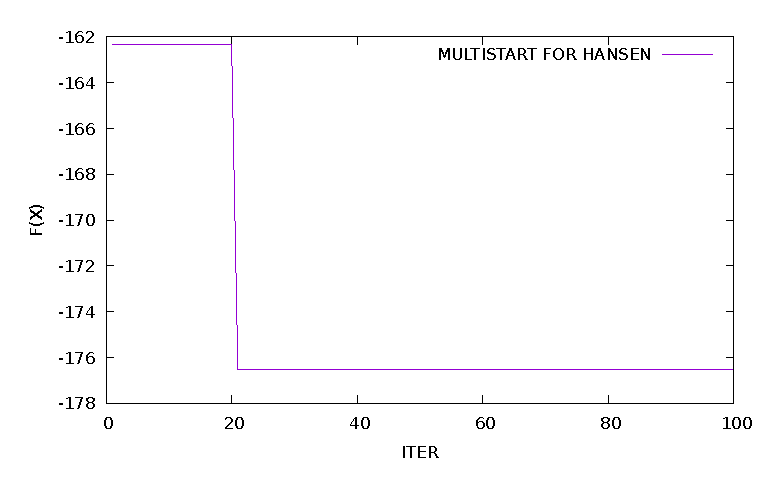
\includegraphics[scale=0.7]{hansen_plot}
\end{figure}
\begin{figure}

\caption{Plot of the used termination rule for the EXP8 test function.\label{fig:exp8_plot}}

\centering{}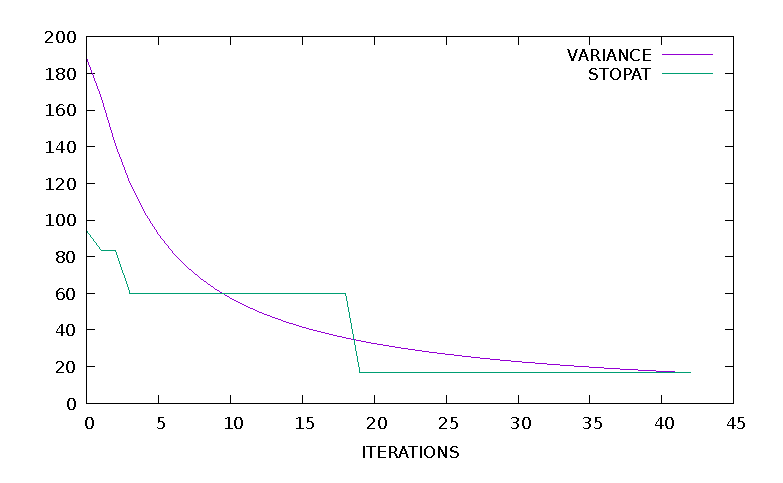
\includegraphics[scale=0.7]{termination_check}
\end{figure}


\subsection{Rbf networks \label{subsec:Rbf-networks}}

An RBF neural network typically is expressed as a function: \textbf{
\begin{equation}
y(\overrightarrow{x})=\sum_{i=1}^{k}w_{i}\phi\left(\left\Vert x-c_{i}\right\Vert \right)\label{eq:firstrbf}
\end{equation}
}where the vector $\overrightarrow{x}$ stands for the input vector
of the network and the vector $\overrightarrow{w}$ is called weight
vector with $k$ elements. Typically, the function $\phi(x)$ is the
so - called Gaussian function defined as:

\textbf{
\begin{equation}
\phi(x)=\exp\left(-\frac{\left(x-c\right)^{2}}{\sigma^{2}}\right)
\end{equation}
}where the value $\phi(x)$ depends mainly on the distance between
$x$ and $x$. The vector $\overrightarrow{c}$ is called centroid
and the vector $\overrightarrow{\sigma}=\left(\sigma_{1},\sigma_{2},\ldots,\sigma_{k}\right)$
is considered as the variance vector. A typical plot of this function
is shown in Figure \ref{fig:gaussianPlot}. 

The network of equation \ref{eq:firstrbf} can be used to approximate
functions $f(x),\ x\in S\subset R^{n}$ by minimizing the error:
\begin{equation}
E\left(y\left(\overrightarrow{x}\right)\right)=\sum_{i=1}^{M}\left(y\left(x_{i}\right)-f\left(x_{i}\right)\right)^{2}\label{eq:rbf_error}
\end{equation}
where the variable $M$ denotes the number of training samples provided
for the function $f(x)$. The RBF network is shown graphically in
Figure \ref{fig:rbfExample}. During a training procedure, the parameters
of the RBF network are adapted in order to minimize the error of equation
\ref{eq:rbf_error} .The RBF network us trained using a two - phase
methodology:
\begin{enumerate}
\item During the first phase the $k$ centers of and the associated variances
are calculated through K-Means algorithm \cite{kmeans}.
\item During the second phase, the weight vector $\overrightarrow{w}=\left(w_{1},w_{2},\ldots,w_{k}\right)$
is calculated by solving a linear system of equations with the following
procedure:
\begin{enumerate}
\item \textbf{Set} \textbf{$W=w_{kj}$},\textbf{ }the matrix for the $k$
weights 
\item \textbf{Set} \textbf{$\Phi=\phi_{j}\left(x_{i}\right)$}
\item \textbf{Set $T=\left\{ t_{i}=f\left(x_{i}\right),i=1,..,M\right\} $. }
\item The system to be solved is defined as:\textbf{ 
\begin{equation}
\Phi^{T}\left(T-\Phi W^{T}\right)=0
\end{equation}
}The solution is:\textbf{
\begin{equation}
W^{T}=\left(\Phi^{T}\Phi\right)^{-1}\Phi^{T}T=\Phi^{\dagger}T\label{eq:eqoutput}
\end{equation}
}The matrix\textbf{ $\Phi^{\dagger}=\left(\Phi^{T}\Phi\right)^{-1}\Phi^{T}$
}is the so - called  pseudo-inverse of $\Phi$, with the property\textbf{
\begin{equation}
\Phi^{\dagger}\Phi=I
\end{equation}
}
\end{enumerate}
\end{enumerate}
In the proposed technique, the previously defined network constructs
an approximation of the objective function $f(x)$ and subsequently
the method Multistart takes samples from the approximation of the
objective function.\textbf{ }The process starts by taking some samples
from the actual $f(x)$ function. These samples are then used to train
an RBF neural network. After training, many samples are taken from
the neural network function and the best ones will be used in the
global optimization method. The overall sampling procedure is shown
in Algorithm \ref{alg:proposedSampling}.

\begin{figure}
\caption{Typical plot of the Gaussian function.\label{fig:gaussianPlot}}

\centering{}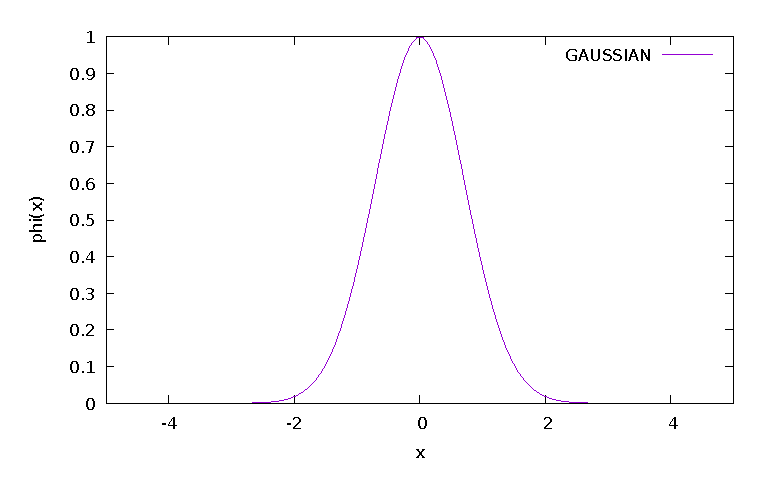
\includegraphics{gaussian}
\end{figure}
\begin{figure}
\caption{An example of an RBF network.\label{fig:rbfExample}}

\centering{}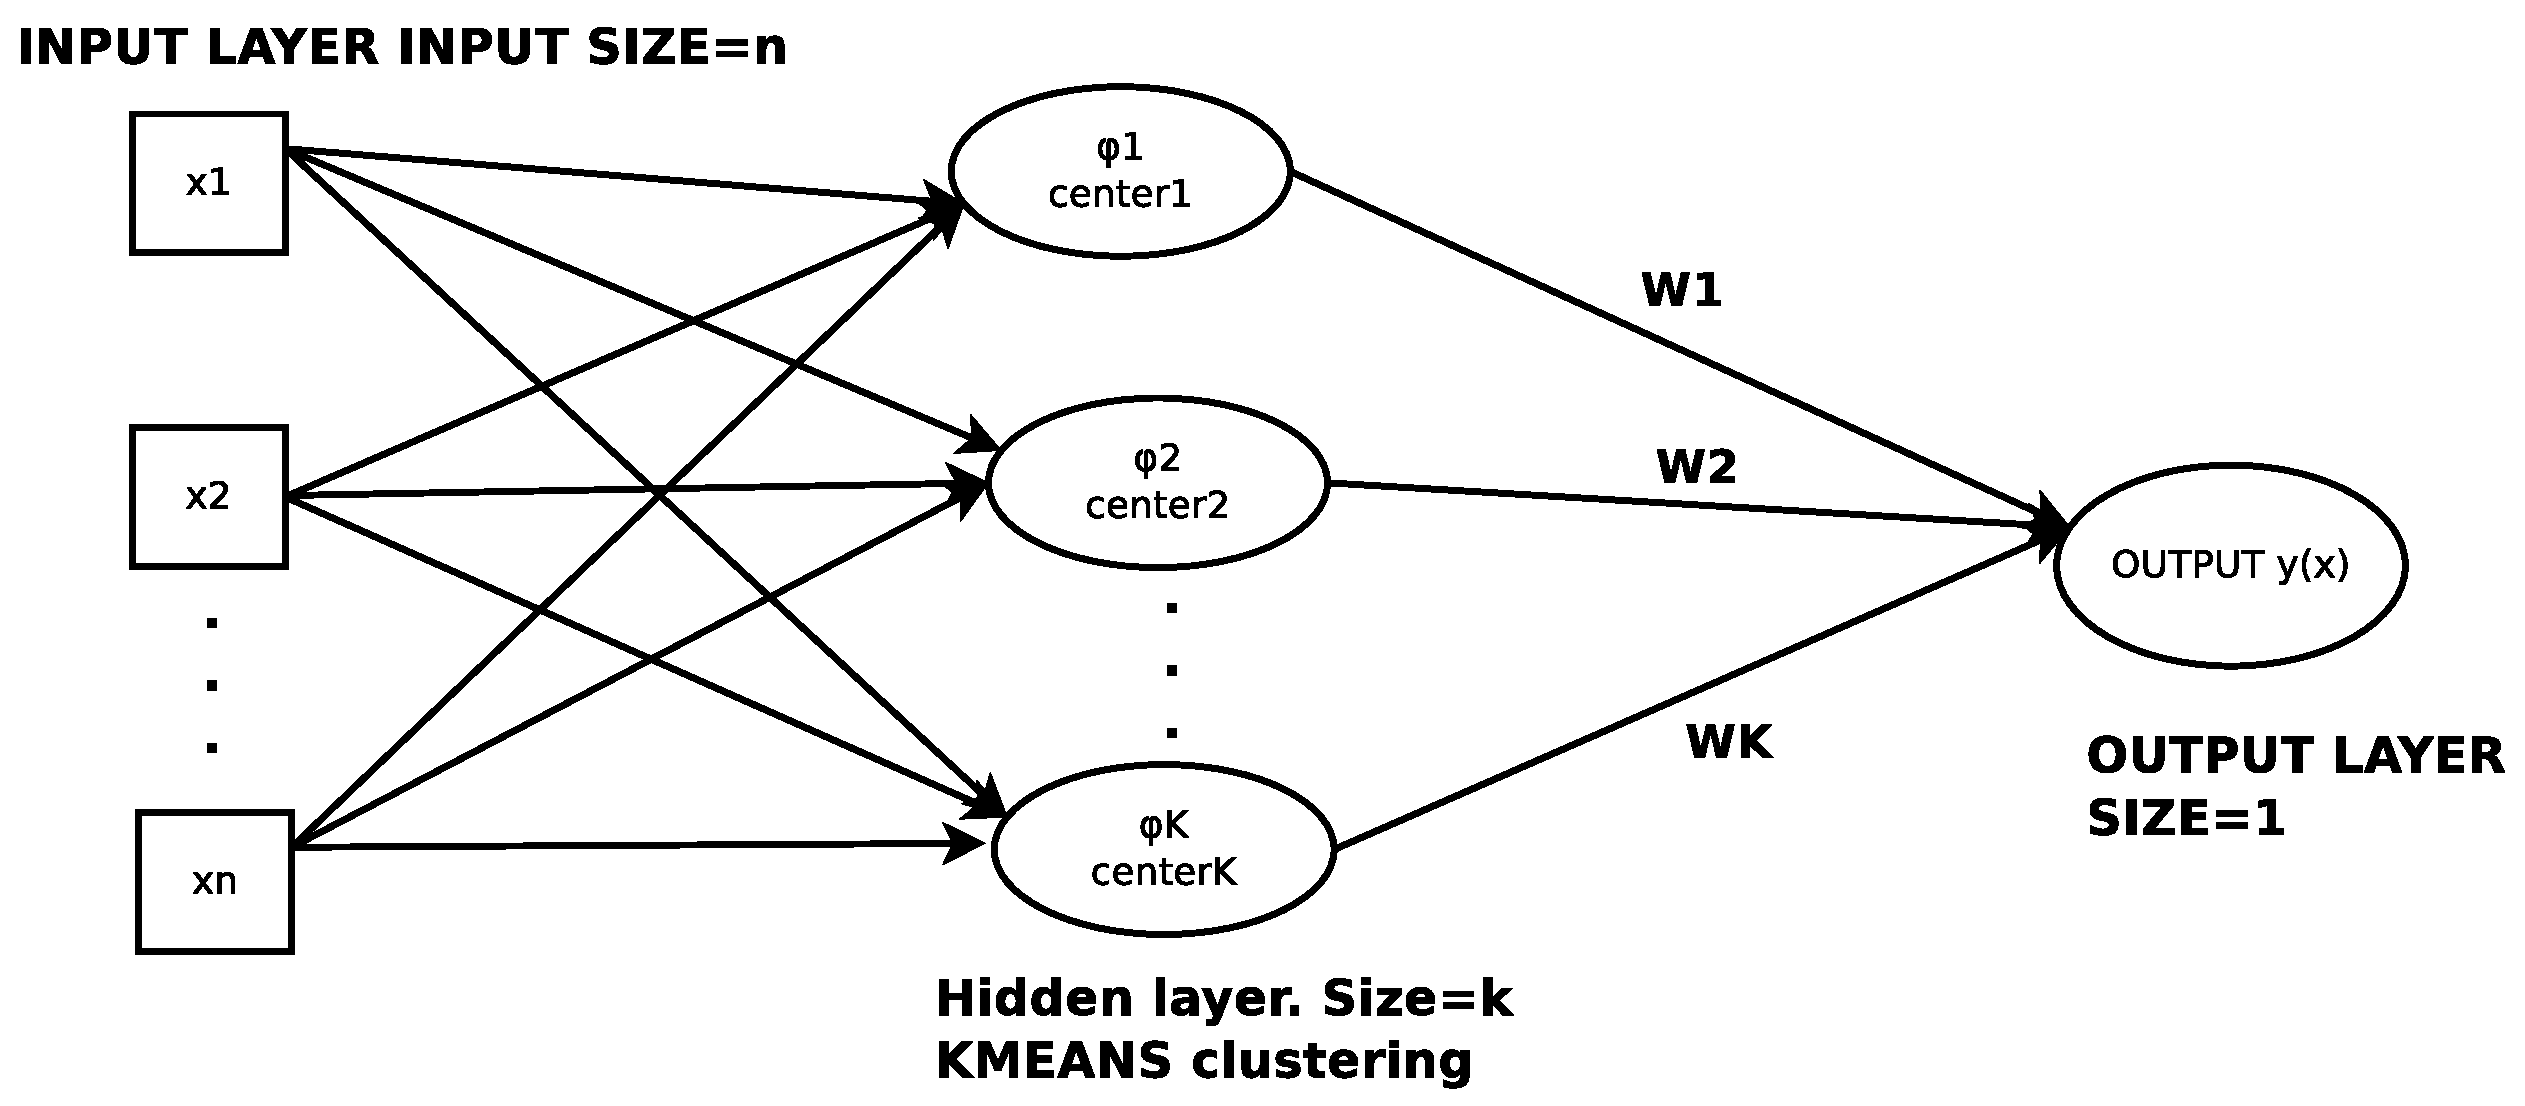
\includegraphics[scale=0.3]{rbfdiagram}
\end{figure}
\begin{algorithm}
\caption{The proposed sampling procedure.\label{alg:proposedSampling}}

\begin{enumerate}
\item \textbf{Initialization} step.
\begin{enumerate}
\item \textbf{Set} $N$, the number of required samples.
\item \textbf{Set} ISAMPLES, the initial samples that will be drawn from
the function $f(x)$.
\item \textbf{Set} $\mbox{FR}$ a real number, with $\text{\mbox{FR} }>N$.
For example, $\mbox{FR}=10\times N$
\item \textbf{Set} $\mbox{IS}=\emptyset$
\item \textbf{Set} $\mbox{FS}=\emptyset$. This is the final outcome of
the algorithm.
\item \textbf{Set} $k$, the number of weights for the RBF network,
\end{enumerate}
\item \textbf{Initial Sampling} step.
\begin{enumerate}
\item \textbf{For} $i=1,\ldots,\mbox{ISAMPLES}$\textbf{do}
\begin{enumerate}
\item Take a sample $s_{i}=\left(x_{i},f\left(x_{i}\right)\right),x_{i}\in S\subset R^{n}$
\item $\mbox{IS}=\mbox{IS}\cup s_{i}$
\end{enumerate}
\item \textbf{End For}
\end{enumerate}
\item \textbf{Training} step.
\begin{enumerate}
\item \textbf{Construct} an RBF network $y(x)$ with $k$ weights. 
\item \textbf{Train} $y(x)$ using the set $\mbox{IS}$ by minimizing the
train error of equation \ref{eq:rbf_error}.
\end{enumerate}
\item \textbf{Final sampling} step.
\begin{enumerate}
\item \textbf{For} $i=1,\ldots,\mbox{FR}$ \textbf{do}
\begin{enumerate}
\item \textbf{Take} a sample $s_{i}=\left(x_{i},y\left(x_{i}\right)\right)$
\item $\mbox{FS}=\mbox{FS}\cup s_{i}$
\end{enumerate}
\item \textbf{End For}
\item \textbf{Sort} FS according to the function values.
\item \textbf{Keep} in the set only the N samples with the lowest functional
value.
\end{enumerate}
\end{enumerate}
\end{algorithm}


\section{Experiments \label{sec:Experiments}}

The effectiveness of the proposed method was evaluated using some
benchmark functions from the relevant literature \cite{Ali1,Floudas1}.

\subsection{Test functions}
\begin{itemize}
\item \textbf{\emph{Bent Cigar function}}\emph{ }The function is 
\[
f(x)=x_{1}^{2}+10^{6}\sum_{i=2}^{n}x_{i}^{2}
\]
 with the global minimum $f\left(x^{*}\right)=0$. For the conducted
experiments the value $n=10$ was used.
\item \textbf{Bf1} function. The function Bohachevsky 1 is given by the
equation
\end{itemize}
\[
f(x)=x_{1}^{2}+2x_{2}^{2}-\frac{3}{10}\cos\left(3\pi x_{1}\right)-\frac{4}{10}\cos\left(4\pi x_{2}\right)+\frac{7}{10}
\]
with $x\in[-100,100]^{2}$. The value of global minimum is 0.0.
\begin{itemize}
\item \textbf{Bf2} function. The function Bohachevsky 2 is given by the
equation 
\[
f(x)=x_{1}^{2}+2x_{2}^{2}-\frac{3}{10}\cos\left(3\pi x_{1}\right)\cos\left(4\pi x_{2}\right)+\frac{3}{10}
\]
with $x\in[-50,50]^{2}$. The value of the global minimum is 0.0.
\item \textbf{Branin} function. The function is defined by $f(x)=\left(x_{2}-\frac{5.1}{4\pi^{2}}x_{1}^{2}+\frac{5}{\pi}x_{1}-6\right)^{2}+10\left(1-\frac{1}{8\pi}\right)\cos(x_{1})+10$
with $-5\le x_{1}\le10,\ 0\le x_{2}\le15$. The value of global minimum
is 0.397887.with $x\in[-10,10]^{2}$. The value of global minimum
is -0.352386.
\item \textbf{CM} function. The Cosine Mixture function is given by the
equation 
\[
f(x)=\sum_{i=1}^{n}x_{i}^{2}-\frac{1}{10}\sum_{i=1}^{n}\cos\left(5\pi x_{i}\right)
\]
with $x\in[-1,1]^{n}$. The value of the global minimum is -0.4 and
in our experiments we have used $n=4$. The corresponding function
is denotes as CM4
\item \textbf{Camel} function. The function is given by 
\[
f(x)=4x_{1}^{2}-2.1x_{1}^{4}+\frac{1}{3}x_{1}^{6}+x_{1}x_{2}-4x_{2}^{2}+4x_{2}^{4},\quad x\in[-5,5]^{2}
\]
The global minimum has the value of $f\left(x^{*}\right)=-1.0316$
\item \textbf{Discus function}\emph{ }The function is defined as 
\[
f(x)=10^{6}x_{1}^{2}+\sum_{i=2}^{n}x_{i}^{2}
\]
 with global minimum $f\left(x^{*}\right)=0.$ For the conducted experiments
the value $n=10$ was used.
\item \textbf{Easom} function The function is given by the equation 
\[
f(x)=-\cos\left(x_{1}\right)\cos\left(x_{2}\right)\exp\left(\left(x_{2}-\pi\right)^{2}-\left(x_{1}-\pi\right)^{2}\right)
\]
with $x\in[-100,100]^{2}$ and global minimum -1.0
\item \textbf{Exponential} function. The function is given by 
\[
f(x)=-\exp\left(-0.5\sum_{i=1}^{n}x_{i}^{2}\right),\quad-1\le x_{i}\le1
\]
The global minimum is located at $x^{*}=(0,0,...,0)$ with value $-1$.
In our experiments we used this function with $n=4,16,64$ and the
corresponding functions are denoted by the labels EXP4, EXP16, EXP64.
\item \textbf{Griewank2} function. The function is given by
\[
f(x)=1+\frac{1}{200}\sum_{i=1}^{2}x_{i}^{2}-\prod_{i=1}^{2}\frac{\cos(x_{i})}{\sqrt{(i)}},\quad x\in[-100,100]^{2}
\]
The global minimum is located at the $x^{*}=(0,0,...,0)$ with value
0.
\item \textbf{Griewank10} function. The function is given by the equation
\[
f(x)=\sum_{i=1}^{n}\frac{x_{i}^{2}}{4000}-\prod_{i=1}^{n}\cos\left(\frac{x_{i}}{\sqrt{i}}\right)+1
\]
In our experiments we have used $n=10$ and the global minimum is
0.0 The function has several local minima in the specified range.
\item \textbf{Hansen} function. $f(x)=\sum_{i=1}^{5}i\cos\left[(i-1)x_{1}+i\right]\sum_{j=1}^{5}j\cos\left[(j+1)x_{2}+j\right]$,
$x\in[-10,10]^{2}$ . The global minimum of the function is -176.541793.
\item \textbf{Hartman 3} function. The function is given by
\[
f(x)=-\sum_{i=1}^{4}c_{i}\exp\left(-\sum_{j=1}^{3}a_{ij}\left(x_{j}-p_{ij}\right)^{2}\right)
\]
with $x\in[0,1]^{3}$ and $a=\left(\begin{array}{ccc}
3 & 10 & 30\\
0.1 & 10 & 35\\
3 & 10 & 30\\
0.1 & 10 & 35
\end{array}\right),\ c=\left(\begin{array}{c}
1\\
1.2\\
3\\
3.2
\end{array}\right)$ and
\[
p=\left(\begin{array}{ccc}
0.3689 & 0.117 & 0.2673\\
0.4699 & 0.4387 & 0.747\\
0.1091 & 0.8732 & 0.5547\\
0.03815 & 0.5743 & 0.8828
\end{array}\right)
\]
The value of global minimum is -3.862782.
\item \textbf{Hartman 6} function.
\[
f(x)=-\sum_{i=1}^{4}c_{i}\exp\left(-\sum_{j=1}^{6}a_{ij}\left(x_{j}-p_{ij}\right)^{2}\right)
\]
with $x\in[0,1]^{6}$ and $a=\left(\begin{array}{cccccc}
10 & 3 & 17 & 3.5 & 1.7 & 8\\
0.05 & 10 & 17 & 0.1 & 8 & 14\\
3 & 3.5 & 1.7 & 10 & 17 & 8\\
17 & 8 & 0.05 & 10 & 0.1 & 14
\end{array}\right),\ c=\left(\begin{array}{c}
1\\
1.2\\
3\\
3.2
\end{array}\right)$ and
\[
p=\left(\begin{array}{cccccc}
0.1312 & 0.1696 & 0.5569 & 0.0124 & 0.8283 & 0.5886\\
0.2329 & 0.4135 & 0.8307 & 0.3736 & 0.1004 & 0.9991\\
0.2348 & 0.1451 & 0.3522 & 0.2883 & 0.3047 & 0.6650\\
0.4047 & 0.8828 & 0.8732 & 0.5743 & 0.1091 & 0.0381
\end{array}\right)
\]
the value of global minimum is -3.322368.
\item \textbf{High Conditioned Elliptic} function, defined as 
\[
f(x)=\sum_{i=1}^{n}\left(10^{6}\right)^{\frac{i-1}{n-1}}x_{i}^{2}
\]
with global minimum $f\left(x^{*}\right)=0$ and the value $n=10$
was used in the conducted experiments
\item \textbf{Potential} function. The molecular conformation corresponding
to the global minimum of the energy of N atoms interacting via the
Lennard-Jones potential\cite{Jones} is used as a test case here.
The function to be minimized is given by:
\begin{equation}
V_{LJ}(r)=4\epsilon\left[\left(\frac{\sigma}{r}\right)^{12}-\left(\frac{\sigma}{r}\right)^{6}\right]\label{eq:potential}
\end{equation}
In the current experiments three different cases were studied: $N=3,\ 5$
\item \textbf{Rastrigin} function. The function is given by 
\[
f(x)=x_{1}^{2}+x_{2}^{2}-\cos(18x_{1})-\cos(18x_{2}),\quad x\in[-1,1]^{2}
\]
The global minimum is located at $x^{*}=(0,0)$ with value -2.0.
\item \textbf{Shekel 7} function.
\end{itemize}
\[
f(x)=-\sum_{i=1}^{7}\frac{1}{(x-a_{i})(x-a_{i})^{T}+c_{i}}
\]

with $x\in[0,10]^{4}$ and $a=\left(\begin{array}{cccc}
4 & 4 & 4 & 4\\
1 & 1 & 1 & 1\\
8 & 8 & 8 & 8\\
6 & 6 & 6 & 6\\
3 & 7 & 3 & 7\\
2 & 9 & 2 & 9\\
5 & 3 & 5 & 3
\end{array}\right),\ c=\left(\begin{array}{c}
0.1\\
0.2\\
0.2\\
0.4\\
0.4\\
0.6\\
0.3
\end{array}\right)$. The value of global minimum is -10.342378.
\begin{itemize}
\item \textbf{Shekel 5 }function.
\end{itemize}
\[
f(x)=-\sum_{i=1}^{5}\frac{1}{(x-a_{i})(x-a_{i})^{T}+c_{i}}
\]
 

with $x\in[0,10]^{4}$ and $a=\left(\begin{array}{cccc}
4 & 4 & 4 & 4\\
1 & 1 & 1 & 1\\
8 & 8 & 8 & 8\\
6 & 6 & 6 & 6\\
3 & 7 & 3 & 7
\end{array}\right),\ c=\left(\begin{array}{c}
0.1\\
0.2\\
0.2\\
0.4\\
0.4
\end{array}\right)$. The value of global minimum is -10.107749.
\begin{itemize}
\item \textbf{Shekel 10} function.
\end{itemize}
\[
f(x)=-\sum_{i=1}^{10}\frac{1}{(x-a_{i})(x-a_{i})^{T}+c_{i}}
\]
 

with $x\in[0,10]^{4}$ and $a=\left(\begin{array}{cccc}
4 & 4 & 4 & 4\\
1 & 1 & 1 & 1\\
8 & 8 & 8 & 8\\
6 & 6 & 6 & 6\\
3 & 7 & 3 & 7\\
2 & 9 & 2 & 9\\
5 & 5 & 3 & 3\\
8 & 1 & 8 & 1\\
6 & 2 & 6 & 2\\
7 & 3.6 & 7 & 3.6
\end{array}\right),\ c=\left(\begin{array}{c}
0.1\\
0.2\\
0.2\\
0.4\\
0.4\\
0.6\\
0.3\\
0.7\\
0.5\\
0.6
\end{array}\right)$. The value of global minimum is -10.536410.
\begin{itemize}
\item \textbf{Sinusoidal} function. The function is given by 
\[
f(x)=-\left(2.5\prod_{i=1}^{n}\sin\left(x_{i}-z\right)+\prod_{i=1}^{n}\sin\left(5\left(x_{i}-z\right)\right)\right),\quad0\le x_{i}\le\pi.
\]
The global minimum is located at $x^{*}=(2.09435,2.09435,...,2.09435)$
with $f\left(x^{*}\right)=-3.5$. In our experiments we used $n=4,8,16$
and $z=\frac{\pi}{6}$ and the corresponding functions are denoted
by the labels SINU4, SINU8 and SINU16 respectively.
\item \textbf{Test2N} function. This function is given by the equation 
\[
f(x)=\frac{1}{2}\sum_{i=1}^{n}x_{i}^{4}-16x_{i}^{2}+5x_{i},\quad x_{i}\in[-5,5].
\]
The function has $2^{n}$ in the specified range and in our experiments
we used $n=4,5,6,7$. The corresponding values of global minimum is
-156.664663 for $n=4$, -195.830829 for $n=5$, -234.996994 for $n=6$
and -274.163160 for $n=7$.
\item \textbf{Test30N} function. This function is given by 
\[
f(x)=\frac{1}{10}\sin^{2}\left(3\pi x_{1}\right)\sum_{i=2}^{n-1}\left(\left(x_{i}-1\right)^{2}\left(1+\sin^{2}\left(3\pi x_{i+1}\right)\right)\right)+\left(x_{n}-1\right)^{2}\left(1+\sin^{2}\left(2\pi x_{n}\right)\right)
\]
with $x\in[-10,10]$. The function has $30^{n}$ local minima in the
specified range and we used $n=3,4$ in our experiments. The value
of global minimum for this function is 0.0
\end{itemize}

\subsection{Experimental results}

The proposed sampling method was tested against the uniform sampling,
for the Multistart global optimization technique. The uniform distribution
used to sample points is defined as:

\begin{equation}
x_{i}=a_{i}+r\times\left(b_{i}-a_{i}\right),\ i=1\ldots n\label{eq:eq4}
\end{equation}
with $r\in[0,1]$ a random number. The parameters for the experiments
are listed in Table \ref{tab:Parameters}. All the experiments were
executed 30 times with different random numbers each time. In all
cases, the stopping rule of subsection \ref{subsec:The-used-termination}
was incorporated. The random number function used was the drand48()
function of the C programming language. The experimental results for
used test functions are listed in Tables \ref{tab:multistart_results},
\ref{tab:proposed20} and \ref{tab:proposed50}. The number in the
cells denotes the average function calls for the 30 independent runs.
The fraction in parentheses stands for the fraction of runs where
the global optimum was found. If this number is missing then the global
minimum was discovered in every independent run (100\% success). At
the end of each table, an additional line named total has been added,
representing the total number of function calls and, in parentheses,
the average success rate in finding the total minimum.

From the experimental results, it follows in principle that the use
of neural networks significantly reduces the required number of function
calls needed to find the total minimum. This reduction is proportional
to the objective function and can reach up to 60\% of the original
number of function calls. In addition, the usage of the ISAMPLES parameter
significantly increases the reliability of the new sampling method.
For example, in the case where N=20 there is an increase in the average
success rate for finding the total minimum from 90\% to approximately
96\%. However, improving the reliability of the method does not imply
an increase in the number of function calls. For example, for N=20
the calls are in the interval $[75000,90000]$ without showing any
clear increase. However, the use of the new sampling technique requires
significantly more computing time than the uniform distribution because
of the need to train the RBF networks and also because of the classification
that precedes taking the final samples. This difference is demonstrated
in Figure \ref{fig:sinuComparison}. In this we see the significant
difference in running time for the SINU problem with a different number
of dimensions each time. 

\begin{table}

\caption{Parameters for the experiments.\label{tab:Parameters}}

\centering{}%
\begin{tabular}{|c|c|}
\hline 
PARAMETER & VALUE\tabularnewline
\hline 
\hline 
$\mbox{ITER}_{\mbox{MAX}}$ & 100\tabularnewline
\hline 
$k$ & 10\tabularnewline
\hline 
$N$ & 20,50\tabularnewline
\hline 
FR & $10\times N$\tabularnewline
\hline 
\end{tabular}
\end{table}

\begin{table}
\caption{Experimental results for the Multistart method, using uniform distribution
for the samples as defined in Equation \ref{eq:eq4}. \label{tab:multistart_results}}

\begin{centering}
\begin{tabular}{|c|c|c|}
\hline 
FUNCTION & N=20 & N=50\tabularnewline
\hline 
\hline 
BF1 & 3004 & 5975\tabularnewline
\hline 
BF2 & 2828 & 5826\tabularnewline
\hline 
BRANIN & 2409 & 5415\tabularnewline
\hline 
CAMEL & 2661 & 5599\tabularnewline
\hline 
CIGAR & 5588 & 8410\tabularnewline
\hline 
CM4 & 3551(0.87) & 6431(0.80)\tabularnewline
\hline 
DISCUS & 2817 & 5965\tabularnewline
\hline 
EASOM & 2204 & 5202\tabularnewline
\hline 
EXP4 & 2769 & 5772\tabularnewline
\hline 
EXP16 & 2836 & 5837\tabularnewline
\hline 
EXP64 & 2912 & 5914\tabularnewline
\hline 
GRIEWANK2 & 3938(0.40) & 6572(0.30)\tabularnewline
\hline 
GRIEWANK10 & 4536(0.97) & 7520\tabularnewline
\hline 
POTENTIAL3 & 3121 & 6120\tabularnewline
\hline 
POTENTIAL5 & 4363 & 7320\tabularnewline
\hline 
HANSEN & 5344(0.93) & 9536(0.90)\tabularnewline
\hline 
HARTMAN3 & 2618 & 5608\tabularnewline
\hline 
HARTMAN6 & 3014 & 6037\tabularnewline
\hline 
HIGHELLIPTIC & 4398 & 7306\tabularnewline
\hline 
RASTRIGIN & 3850(0.83) & 6401(0.77)\tabularnewline
\hline 
ROSENBROCK4 & 6456 & 8584\tabularnewline
\hline 
ROSENBROCK8 & 7646 & 10095\tabularnewline
\hline 
SHEKEL5 & 3144 & 6215\tabularnewline
\hline 
SHEKEL7 & 3354 & 6508\tabularnewline
\hline 
SHEKEL10 & 3388 & 6860\tabularnewline
\hline 
SINU4 & 3935 & 6670(0.97)\tabularnewline
\hline 
SINU8 & 5547 & 8056\tabularnewline
\hline 
SINU16 & 19313 & 35751(0.97)\tabularnewline
\hline 
TEST2N4 & 3035(0.87) & 6002(0.97)\tabularnewline
\hline 
TEST2N5 & 3127(0.73) & 6042(0.67)\tabularnewline
\hline 
TEST2N6 & 3393(0.40) & 6169(0.47)\tabularnewline
\hline 
TEST2N7 & 4075(0.37) & 6443(0.33)\tabularnewline
\hline 
TEST30N3 & 3723 & 6322\tabularnewline
\hline 
TEST30N4 & 3736 & 6465\tabularnewline
\hline 
\textbf{TOTAL} & \textbf{142632(0.923)} & \textbf{254988(0.916)}\tabularnewline
\hline 
\end{tabular}
\par\end{centering}
\end{table}
\begin{table}
\caption{Experimental results for the proposed method with N=20\label{tab:proposed20}}

\centering{}%
\begin{tabular}{|c|c|c|c|}
\hline 
FUNCTION & ISAMPLES=100 & ISAMPLES=200 & ISAMPLES=500\tabularnewline
\hline 
\hline 
BF1 & 1086 & 1159 & 1500\tabularnewline
\hline 
BF2 & 922 & 1026 & 1304\tabularnewline
\hline 
BRANIN & 503 & 590 & 899\tabularnewline
\hline 
CAMEL & 670 & 756 & 1060\tabularnewline
\hline 
CIGAR & 3482 & 3236 & 2849\tabularnewline
\hline 
CM4 & 1583(0.83) & 1716(0.83) & 1861(0.90)\tabularnewline
\hline 
DISCUS & 931 & 1206 & 1525\tabularnewline
\hline 
EASOM & 1063 & 401 & 704\tabularnewline
\hline 
EXP4 & 766 & 803 & 1049\tabularnewline
\hline 
EXP16 & 912 & 1009 & 1303\tabularnewline
\hline 
EXP64 & 968 & 1070 & 1359\tabularnewline
\hline 
GRIEWANK2 & 2409(0.53) & 1641(0.40) & 2069(0.57)\tabularnewline
\hline 
GRIEWANK10 & 2607(0.97) & 2609 & 2902(0.93)\tabularnewline
\hline 
POTENTIAL3 & 1211 & 1297 & 1613\tabularnewline
\hline 
POTENTIAL5 & 2414 & 2521 & 2835\tabularnewline
\hline 
HANSEN & 6079(0.87) & 4785(0.83) & 6504(0.77)\tabularnewline
\hline 
HARTMAN3 & 729 & 830 & 1143\tabularnewline
\hline 
HARTMAN6 & 1111(0.90) & 1290(0.93) & 1525(0.97)\tabularnewline
\hline 
HIGHELLIPTIC & 2618 & 2671 & 3098\tabularnewline
\hline 
RASTRIGIN & 1727(0.57) & 1043(0.87) & 1386\tabularnewline
\hline 
ROSENBROCK4 & 4111 & 2672 & 4357\tabularnewline
\hline 
ROSENBROCK8 & 5417 & 6253 & 5609\tabularnewline
\hline 
SHEKEL5 & 1751(0.73) & 2152(0.90) & 1245(0.90)\tabularnewline
\hline 
SHEKEL7 & 1667(0.87) & 1627(0.83) & 1676(0.93)\tabularnewline
\hline 
SHEKEL10 & 2329(0.80) & 2946(0.73) & 3678(0.77)\tabularnewline
\hline 
SINU4 & 938 & 991 & 1227\tabularnewline
\hline 
SINU8 & 1194 & 1360 & 1479\tabularnewline
\hline 
SINU16 & 14305(0.87) & 32647(0.97) & 21363(0.97)\tabularnewline
\hline 
TEST2N4 & 904(0.57) & 936(0.73) & 1227\tabularnewline
\hline 
TEST2N5 & 1881(0.80) & 1218 & 1351\tabularnewline
\hline 
TEST2N6 & 1092(0.67) & 1224(0.87) & 1435(0.97)\tabularnewline
\hline 
TEST2N7 & 1452(0.70) & 1397(0.80) & 1477(0.90)\tabularnewline
\hline 
TEST30N3 & 1244 & 2054 & 2584\tabularnewline
\hline 
TEST30N4 & 2027 & 2644 & 2638\tabularnewline
\hline 
\textbf{TOTAL} & \textbf{74103(0.902)} & \textbf{91780(0.932)} & \textbf{89834(0.958)}\tabularnewline
\hline 
\end{tabular}
\end{table}
\begin{table}
\caption{Experimental results for the proposed method with N=50\label{tab:proposed50}}

\centering{}%
\begin{tabular}{|c|c|c|c|}
\hline 
FUNCTION & ISAMPLES=100 & ISAMPLES=200 & ISAMPLES=500\tabularnewline
\hline 
\hline 
BF1 & 1093 & 1175 & 1527\tabularnewline
\hline 
BF2 & 943 & 1022 & 1319\tabularnewline
\hline 
BRANIN & 502(0.97) & 594 & 900\tabularnewline
\hline 
CAMEL & 642 & 729 & 1046\tabularnewline
\hline 
CIGAR & 3527 & 3228 & 6729\tabularnewline
\hline 
CM4 & 1491(0.87) & 1884(0.90) & 1799(0.97)\tabularnewline
\hline 
DISCUS & 828 & 1365 & 1215\tabularnewline
\hline 
EASOM & 2320 & 398 & 723\tabularnewline
\hline 
EXP4 & 766 & 827 & 1050\tabularnewline
\hline 
EXP16 & 912 & 1007 & 1298\tabularnewline
\hline 
EXP64 & 983 & 1064 & 1358\tabularnewline
\hline 
GRIEWANK2 & 1788(0.50) & 1762(0.43) & 2345(0.50)\tabularnewline
\hline 
GRIEWANK10 & 2505 & 2677 & 2868\tabularnewline
\hline 
POTENTIAL3 & 1244 & 1313 & 1609\tabularnewline
\hline 
POTENTIAL5 & 2420 & 2502 & 2795\tabularnewline
\hline 
HANSEN & 6711(0.70) & 4278(0.70) & 7264(0.67)\tabularnewline
\hline 
HARTMAN3 & 728 & 830 & 1144\tabularnewline
\hline 
HARTMAN6 & 1027(0.93) & 1202(0.93) & 1492\tabularnewline
\hline 
HIGHELLIPTIC & 3455 & 2889 & 3078\tabularnewline
\hline 
RASTRIGIN & 977(0.53) & 1269(0.77) & 1397(0.97)\tabularnewline
\hline 
ROSENBROCK4 & 2348 & 2453 & 3278\tabularnewline
\hline 
ROSENBROCK8 & 3928 & 4461 & 4865\tabularnewline
\hline 
SHEKEL5 & 5630(0.67) & 7498(0.87) & 1510(0.93)\tabularnewline
\hline 
SHEKEL7 & 2135(0.67) & 1973(0.67) & 1815(0.97)\tabularnewline
\hline 
SHEKEL10 & 1864(0.73) & 1245(0.60) & 3165(0.83)\tabularnewline
\hline 
SINU4 & 984 & 1020 & 1355\tabularnewline
\hline 
SINU8 & 10502 & 1517 & 1456\tabularnewline
\hline 
SINU16 & 95225(0.83) & 21658(0.90) & 21330(0.87)\tabularnewline
\hline 
TEST2N4 & 820(0.63) & 1079(0.90) & 1274\tabularnewline
\hline 
TEST2N5 & 1140(0.67) & 1107(0.80) & 1333\tabularnewline
\hline 
TEST2N6 & 1203(0.73) & 1371(0.97) & 1440(0.97)\tabularnewline
\hline 
TEST2N7 & 1602(0.50) & 1200(0.77) & 1618(0.97)\tabularnewline
\hline 
TEST30N3 & 1494 & 1903 & 2279\tabularnewline
\hline 
TEST30N4 & 1164 & 2287 & 2284\tabularnewline
\hline 
\textbf{TOTAL} & \textbf{164901(0.880)} & \textbf{82787(0.918)} & \textbf{91958(0.960)}\tabularnewline
\hline 
\end{tabular}
\end{table}
\begin{figure}

\caption{Comparison of execution times for the SINU function between the uniform
sampling and the proposed method.\label{fig:sinuComparison}}

\centering{}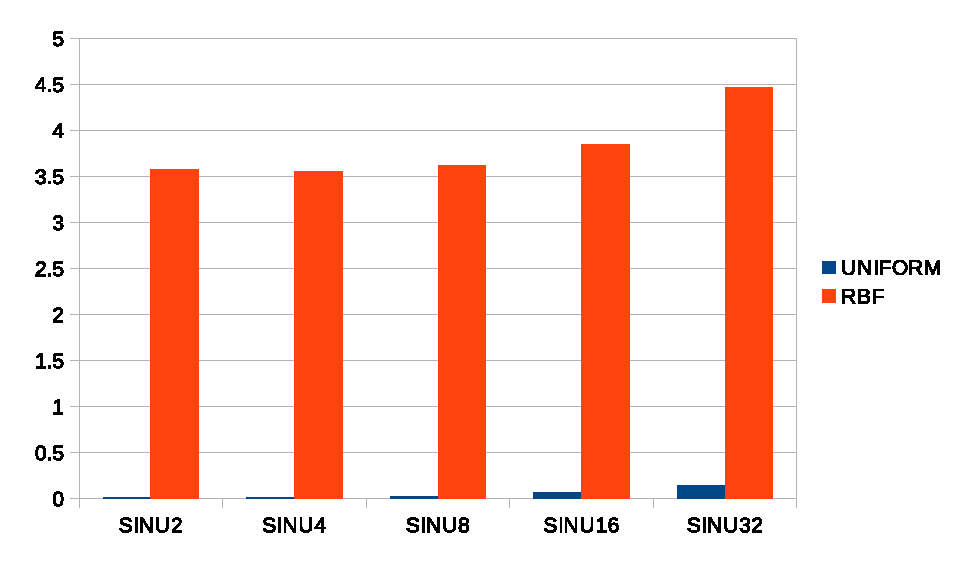
\includegraphics[scale=0.7]{timeforsinu}
\end{figure}


\section{Conclusions \label{sec:Conclusions}}

In this paper, an innovative sampling technique was proposed for the
Multistart global optimization method. The new technique improves
on using a limited number of samples from the objective function in
order to construct an estimator of the function. The estimator in
the present work was an RBF neural network. After the neural network
is trained, a large number of samples are taken from the estimator
without using the objective function anymore. Of these samples, only
those with the lowest functional value of the estimator are used by
the global optimization method. From the experiments performed on
a wide range of objective functions, many of which had a large number
of dimensions, it appears that the proposed technique significantly
outperforms the traditionally used uniform sampling. The gain in the
number of calls in many cases exceeds 60\%. Nevertheless, the new
technique requires more computational time than the uniform distribution,
since it is required to train the network as well as to classify a
series of samples from it. However, this increase in time could be
significantly reduced with the potential use of parallel computing
techniques to train neural networks. Moreover, in large computational
problems, where the cost of evaluating the objective function is extremely
large, the training time of a neural network will be almost negligible.
Future research may include:
\begin{enumerate}
\item Application of the proposed technique to other more efficient global
optimization methods.
\item Parallelization of the training method for the neural network.
\item Usage of more efficient methods to train the RBF networks such as
Genetic Algorithms.
\end{enumerate}
\begin{thebibliography}{10}
\bibitem{global_econ1}Zwe-Lee Gaing, Particle swarm optimization
to solving the economic dispatch considering the generator constraints,
IEEE Transactions on \textbf{18} Power Systems, pp. 1187-1195, 2003.

\bibitem{global_econ2}C. D. Maranas, I. P. Androulakis, C. A. Floudas,
A. J. Berger, J. M. Mulvey, Solving long-term financial planning problems
via global optimization, Journal of Economic Dynamics and Control
\textbf{21}, pp. 1405-1425, 1997.

\bibitem{global_econ3}J. Gao, F. You, Shale Gas Supply Chain Design
and Operations toward Better Economic and Life Cycle Environmental
Performance: MINLP Model and Global Optimization Algorithm, ACS Sustainable
Chem. Eng. \textbf{3}, pp. 1282--1291, 2015.

\bibitem{global_physics1}Q. Duan, S. Sorooshian, V. Gupta, Effective
and efficient global optimization for conceptual rainfall-runoff models,
Water Resources Research \textbf{28}, pp. 1015-1031 , 1992.

\bibitem{global_physics2}P. Charbonneau, Genetic Algorithms in Astronomy
and Astrophysics, Astrophysical Journal Supplement \textbf{101}, p.
309, 1995

\bibitem{global_physics3}T. Gu, W. Luo, H. Xiang, Prediction of two-dimensional
materials by the global optimization approach, WIREs Computational
Molecular Science \textbf{7}, e1295, 2017.

\bibitem{global_chemistry1}A. Liwo, J. Lee, D.R. Ripoll, J. Pillardy,
H. A. Scheraga, Protein structure prediction by global optimization
of a potential energy function, Biophysics \textbf{96}, pp. 5482-5485,
1999.

\bibitem{global_chemistry2}P.M. Pardalos, D. Shalloway, G. Xue, Optimization
methods for computing global minima of nonconvex potential energy
functions, Journal of Global Optimization \textbf{4}, pp. 117-133,
1994.

\bibitem{global_chemistry3}S. Heiles, R.L. Johnston, Global optimization
of clusters using electronic structure methods, Int. J. Quantum Chem.
\textbf{113}, pp. 2091-2109, 2013.

\bibitem{global_med1}Eva K. Lee, Large-Scale Optimization-Based Classification
Models in Medicine and Biology, Annals of Biomedical Engineering \textbf{35},
pp 1095-1109, 2007.

\bibitem{global_med2}Y. Cherruault, Global optimization in biology
and medicine, Mathematical and Computer Modelling \textbf{20}, pp.
119-132, 1994.

\bibitem{interval1}M.A. Wolfe, Interval methods for global optimization,
Applied Mathematics and Computation \textbf{75}, pp. 179-206, 1996.

\bibitem{interval2}T. Csendes and D. Ratz, Subdivision Direction
Selection in Interval Methods for Global Optimization, SIAM J. Numer.
Anal. \textbf{34}, pp. 922--938, 1997. 

\bibitem{interval3}I. Araya, V. Reyes, Interval Branch-and-Bound
algorithms for optimization and constraint satisfaction: a survey
and prospects, J Glob Optim \textbf{65}, pp. 837--866, 2016.

\bibitem{crs1}W. L. Price, Global optimization by controlled random
search, Journal of Optimization Theory and Applications \textbf{40},
pp. 333-348, 1983.

\bibitem{crs2}Ivan K\v{r}iv�, Josef Tvrd�k, The controlled random
search algorithm in optimizing regression models, Computational Statistics
\& Data Analysis \textbf{20}, pp. 229-234, 1995.

\bibitem{crs3}P. Kaelo, M. M. Ali, Numerical studies of some generalized
controlled random search algorithms, Asia-Pacific Journal of Operational
Research 29, 2012.

\bibitem{simann_major}S. Kirkpatrick, CD Gelatt, , MP Vecchi, Optimization
by simulated annealing, Science \textbf{220}, pp. 671-680, 1983.

\bibitem{simann1}B. Suman, P. Kumar, A survey of simulated annealing
as a tool for single and multiobjective optimization, J Oper Res Soc
\textbf{57}, pp. 1143--1160, 2006.

\bibitem{de1}F. Neri, V. Tirronen, Recent advances in differential
evolution: a survey and experimental analysis, Artif Intell Rev \textbf{33},
pp. 61--106, 2010.

\bibitem{de2}S. Das, P. N. Suganthan, Differential Evolution: A Survey
of the State-of-the-Art, IEEE Transactions on Evolutionary Computation
\textbf{15}, pp. 4-31, 2011.

\bibitem{ga1}D. Goldberg, Genetic Algorithms in Search, Optimization
and Machine Learning, Addison-Wesley Publishing Company, Reading,
Massachussets, 1989.

\bibitem{ga2}Z. Michaelewicz, Genetic Algorithms + Data Structures
= Evolution Programs. Springer - Verlag, Berlin, 1996.

\bibitem{ga3}S.A. Grady, M.Y. Hussaini, M.M. Abdullah, Placement
of wind turbines using genetic algorithms, Renewable Energy \textbf{30},
pp. 259-270, 2005.

\bibitem{pso1}Riccardo Poli, James Kennedy kennedy, Tim Blackwell,
Particle swarm optimization An Overview, Swarm Intelligence \textbf{1},
pp 33-57, 2007. 

\bibitem{pso2}Ioan Cristian Trelea, The particle swarm optimization
algorithm: convergence analysis and parameter selection, Information
Processing Letters \textbf{85}, pp. 317-325, 2003.

\bibitem{aco1}M. Dorigo, M. Birattari and T. Stutzle, Ant colony
optimization, IEEE Computational Intelligence Magazine \textbf{1},
pp. 28-39, 2006.

\bibitem{aco2}K. Socha, M. Dorigo, Ant colony optimization for continuous
domains, European Journal of Operational Research 185, pp. 1155-1173,
2008.

\bibitem{pso_sa_hybrid1}H.L. Shieh, C.C. Kuo, C.M. Chiang, Modified
particle swarm optimization algorithm with simulated annealing behavior
and its numerical verification, Applied Mathematics and Computation
\textbf{218}, pp. 4365-4383, 2011.

\bibitem{pso_sa_hybrid2}S. Zhoua, X. Liu, Y. Hua, X. Zhou, S.Yang,
Adaptive model parameter identification for lithium-ion batteries
based on improved coupling hybrid adaptive particle swarm optimization-
simulated annealing method, Journal of Power Sources \textbf{482},
Article number 228951, 2021.

\bibitem{ga_de_hybrid1}D. He, F. Wang, Z. Mao, A hybrid genetic algorithm
approach based on differential evolution for economic dispatch with
valve-point effect, International Journal of Electrical Power \& Energy
Systems \textbf{30}, pp. 31-38, 2008.

\bibitem{ga_de_hybrid2}A. Trivedi, D. Srinivasan, S. Biswas, T. Reindl,
A genetic algorithm -- differential evolution based hybrid framework:
Case study on unit commitment scheduling problem, Information Sciences
\textbf{354}, pp. 275-300, 2016.

\bibitem{ga_pso_hybrid1}Y.T. Kao, E. Zahara, A hybrid genetic algorithm
and particle swarm optimization for multimodal functions, Applied
Soft Computing \textbf{8}, pp. 849-857, 2008.

\bibitem{gpu1}Y. Zhou, Y. Tan, GPU-based parallel particle swarm
optimization, 2009 IEEE Congress on Evolutionary Computation, pp.
1493-1500, 2009.

\bibitem{gpu2}L. Dawson, I. Stewart, Improving Ant Colony Optimization
performance on the GPU using CUDA, in: 2013 IEEE Congress on Evolutionary
Computation, pp. 1901-1908, 2013.

\bibitem{gpu3}Barkalov, K., Gergel, V. Parallel global optimization
on GPU. J Glob Optim \textbf{66}, pp. 3--20, 2016.

\bibitem{multistart-tsp}Li W., A Parallel Multi-start Search Algorithm
for Dynamic Traveling Salesman Problem. In: Pardalos P.M., Rebennack
S. (eds) Experimental Algorithms. SEA 2011. Lecture Notes in Computer
Science, vol 6630. Springer, Berlin, Heidelberg, 2011.

\bibitem{multistart-vehicle}Olli Br�ysy, Geir Hasle, Wout Dullaert,
A multi-start local search algorithm for the vehicle routing problem
with time windows, European Journal of Operational Research \textbf{159},
pp. 586-605, 2004.

\bibitem{multistart_fac}Mauricio G.C. Resende, Renato F. Werneck,A
hybrid multistart heuristic for the uncapacitated facility location
problem, European Journal of Operational Research \textbf{174}, pp.
54-68, 2006.

\bibitem{multistart_clique}E. Marchiori, Genetic, Iterated and Multistart
Local Search for the Maximum Clique Problem. In: Cagnoni S., Gottlieb
J., Hart E., Middendorf M., Raidl G.R. (eds) Applications of Evolutionary
Computing. EvoWorkshops 2002. Lecture Notes in Computer Science, vol
2279. Springer, Berlin, Heidelberg. 

\bibitem{multistart_fire}Gomes M.I., Afonso L.B., Chibeles-Martins
N., Fradinho J.M. (2018) Multi-start Local Search Procedure for the
Maximum Fire Risk Insured Capital Problem. In: Lee J., Rinaldi G.,
Mahjoub A. (eds) Combinatorial Optimization. ISCO 2018. Lecture Notes
in Computer Science, vol 10856. Springer, Cham. https://doi.org/10.1007/978-3-319-96151-4\_19

\bibitem{multistart-aero}Streuber, Gregg M. and Zingg, David. W.,
Evaluating the Risk of Local Optima in Aerodynamic Shape Optimization,
AIAA Journal \textbf{59}, pp. 75-87, 2012.

\bibitem{tmlsl}M.M. Ali, C. Storey, Topographical multilevel single
linkage, J. Global Optimization \textbf{5}, pp. 349--358,1994

\bibitem{Salhi}S. Salhi, N.M. Queen, A hybrid algorithm for identifying
global and local minima when optimizing functions with many minima,
European J. Oper. Res. \textbf{155}, pp. 51--67, 2004.

\bibitem{minfinder}I. G. Tsoulos and I. E. Lagaris, MinFinder: Locating
all the local minima of a function, Computer Physics Communications
\textbf{174}, pp. 166-179, 2006. 

\bibitem{mshybrid1}M. Perez, F. Almeida and J. M. Moreno-Vega, \textquotedbl Genetic
algorithm with multistart search for the p-Hub median problem,\textquotedbl{}
Proceedings. 24th EUROMICRO Conference (Cat. No.98EX204), Vasteras,
Sweden, 1998, pp. 702-707 vol.2.

\bibitem{mshybrid2}H. C. B. d. Oliveira, G. C. Vasconcelos and G.
B. Alvarenga, \textquotedbl A Multi-Start Simulated Annealing Algorithm
for the Vehicle Routing Problem with Time Windows,\textquotedbl{}
2006 Ninth Brazilian Symposium on Neural Networks (SBRN'06), Ribeirao
Preto, Brazil, 2006, pp. 137-142.

\bibitem{grasp}Festa P., Resende M.G.C. (2009) Hybrid GRASP Heuristics.
In: Abraham A., Hassanien AE., Siarry P., Engelbrecht A. (eds) Foundations
of Computational Intelligence Volume 3. Studies in Computational Intelligence,
vol 203. Springer, Berlin, Heidelberg. 

\bibitem{msstop1}B. Betro`, F. Schoen, Optimal and sub-optimal stopping
rules for the multistart algorithm in global optimization, Math. Program.
\textbf{57}, pp. 445--458, 1992.

\bibitem{msstop2}W.E. Hart, Sequential stopping rules for random
optimization methods with applications to multistart local search,
Siam J. Optim. \textbf{9}, pp. 270--290, 1998.

\bibitem{msstop3}I.E. Lagaris and I.G. Tsoulos, Stopping Rules for
Box-Constrained Stochastic Global Optimization, Applied Mathematics
and Computation \textbf{197}, pp. 622-632, 2008.

\bibitem{parallel-multistart}J. Larson and S.M. Wild, Asynchronously
parallel optimization solver for finding multiple minima, Mathematical
Programming Computation \textbf{10}, pp. 303-332, 2018.

\bibitem{parallel-multistart2}H.P.J. Bolton, J.F. Schutte, A.A. Groenwold,
Multiple Parallel Local Searches in Global Optimization. In: Dongarra
J., Kacsuk P., Podhorszki N. (eds) Recent Advances in Parallel Virtual
Machine and Message Passing Interface. EuroPVM/MPI 2000. Lecture Notes
in Computer Science, vol 1908. Springer, Berlin, Heidelberg, 2000.

\bibitem{rbf1}J. Park and I. W. Sandberg, Universal Approximation
Using Radial-Basis-Function Networks, Neural Computation \textbf{3},
pp. 246-257, 1991.

\bibitem{rbf_face}M.J. Er, S. Wu, J. Lu, H.L. Toh, Face recognition
with radial basis function (RBF) neural networks, IEEE Transactions
on Neural Networks \textbf{ 13}, pp. 697-710, 2002.

\bibitem{rbf_function}G.B. Huang, P. Saratchandran, N. Sundararajan,
A generalized growing and pruning RBF (GGAP-RBF) neural network for
function approximation, IEEE Transactions on Neural Networks \textbf{16},
pp. 57-67, 2005.

\bibitem{rbf_image}B.C. Kuo, H.H. Ho, C. H. Li, C. C. Hung , J. S.
Taur, A Kernel-Based Feature Selection Method for SVM With RBF Kernel
for Hyperspectral Image Classification, IEEE Journal of Selected Topics
in Applied Earth Observations and Remote Sensing. \textbf{7}, pp.
317-326, 2014.

\bibitem{rbf_water}H.G. Han, Q.L. Chen, J.F. Qiao, An efficient self-organizing
RBF neural network for water quality prediction, Neural Networks \textbf{24},
pp. 717-725, 2011.

\bibitem{powell}M.J.D Powell, A Tolerant Algorithm for Linearly Constrained
Optimization Calculations, Mathematical Programming \textbf{45}, pp.
547-566, 1989. 

\bibitem{ga_tsoulos}I.G. Tsoulos, Modifications of real code genetic
algorithm for global optimization, Applied Mathematics and Computation
\textbf{203}, pp. 598-607, 2008.

\bibitem{pso_tsoulos}I.G. Tsoulos, A. Tzallas, E. Karvounis, Improving
the PSO method for global optimization problems. Evolving Systems
\textbf{12}, pp. 875--883, 2021

\bibitem{kmeans}MacQueen, J.: Some methods for classification and
analysis of multivariate observations, in: Proceedings of the fifth
Berkeley symposium on mathematical statistics and probability, Vol.
1, No. 14, pp. 281-297, 1967. 

\bibitem{Ali1}M. Montaz Ali, Charoenchai Khompatraporn, Zelda B.
Zabinsky, A Numerical Evaluation of Several Stochastic Algorithms
on Selected Continuous Global Optimization Test Problems, Journal
of Global Optimization \textbf{31}, pp 635-672, 2005. 

\bibitem{Floudas1}C.A. Floudas, P.M. Pardalos, C. Adjiman, W. Esposoto,
Z. G$\ddot{\mbox{u}}$m$\ddot{\mbox{u}}$s, S. Harding, J. Klepeis,
C. Meyer, C. Schweiger, Handbook of Test Problems in Local and Global
Optimization, Kluwer Academic Publishers, Dordrecht, 1999.

\bibitem{Jones}J.E. Lennard-Jones, On the Determination of Molecular
Fields, Proc. R. Soc. Lond. A \textbf{ 106}, pp. 463--477, 1924.
\end{thebibliography}

\end{document}
